\thispagestyle{plain}

\section{Theory}

\subsection{Term Frequency-Inverse Document Frequency}

TF-IDF, as the name suggests, has two components: Term Frequency and Inverse Document Frequency and both are weights assigned to a given term. The former, as \cite{manning2008introduction} defines it, is "equal to the number of occurrences of term \textit{t} in document \textit{d}", or simply denoted by  $\textrm{tf}_{t,d}$.  The latter, on the other hand,  is weight designed to attenuate the \textit{tf} score of  overly common words that possibly have no meaningful importance given a set of documents, e.g. the word \textit{game} in a collection of video game reviews has no impact in discriminating these reviews from one another: Is it talking about \textit{Super Mario} or \textit{Tetris}? IDF is defined by Equation~\ref{eqn:idf}.

\begin{equation}
	\label{eqn:idf}
	idf_t = \log \frac{N}{df_t}
\end{equation}

Where N is the total number of documents and $\textrm{df}_{t}$ is the term's document frequency, i.e. the number of documents that term is in.

Finally, TF-IDF is defined in Equation~\ref{eqn:tfidf} as the product of TF and IDF \citep{manning2008introduction}. It assigns to each term  in a corpus a value that indicates how "important" this word is based on the frequency of said term in each document, TF,  and how rare documents containing said word are, IDF \citep{manning2008introduction}. This method, however, has limitations as it only takes into account term frequencies; it does not capture semantic similarities between words. In addition to that, the TF-IDF representation is normally large and sparse, which can be troublesome for huge corpora \citep{kuhlmann-lec2-2020}.

\begin{equation}
	\label{eqn:tfidf}
	\textrm{tf-idf}_t = \textrm{tf}_{t,d} \times \textrm{idf}_t
\end{equation}


\subsection{Word2Vec: Continuous-Bag-of-Words}

The main goal of Word2Vec is to produce numerical representations of words such that similar words are closer to each other and dissimilar words are far apart. There are two models inside the Word2Vec family: Continuous-Bag-of-Words (CBOW) and skip-gram. This report will focus on the former \footnote{Note: this theory explanation was based on \citep{ghodsi20171} and \citep{ghodsi20172}.}

The main objective of CBOW is to predict a target word  $w_t$ based on surrounding words in a given window, called context words $w_{t-m}, w_{t-m + 1}, ... ,w_{t-1}, w_{t+1}, ..., w_{t+m-1}, w_{t+m}$, where $m$ is the windows size.

The context words are first encoded into one-hot vectors $x_{t-m}, x_{t-m + 1}, ... ,x_{t-1}, x_{t+1}, ..., x_{t+m-1}, x_{t+m}$. The dimension of each vector is [$d \times1$] where $d$ is the number of words in the vocabulary.

Next, all context words are averaged by a  matrix os weights $\mathbf{W}$ such that a overall context vector $v_c$ is extracted.
 
\begin{equation}
	\label{eqn:hidden}
	v_c= \mathbf{W}^T \mathbf{x}
\end{equation}

The context vector $v_c$, sequentially, gets projected back into a d dimensional space via a different weight matrix $\mathbf{W'}$. This new vector is named $u$. 

\begin{equation}
	\label{eqn:hidden2}
	u = \mathbf{W'}^T v_c
\end{equation}

Each entry of this vector, $u_i$ can be written as the product of a word vector $v_w$ times the context vector $v_c$:

\begin{equation}
	\label{eqn:hidden3}
	u_i = v_w^T v_c
\end{equation}

Finally, the vector u is fed to a softmax layer where the output vector $y$ is obtained, which is a probability vector such that it respects Equation~\ref{eqn:w2prob}. Each entry $y_i$ is the probability of a word given the context as seen on Equation~\ref{probs}.

\begin{equation}
	\label{eqn:w2prob}
	\sum_i y_i = 1
\end{equation}

\begin{equation}
	\label{probs}
	y_i = p(w|c) = \textnormal{softmax}(u_i) = \frac{e^{v^T _cv_w}}{\sum_w e^{v^T _cv_w}}
\end{equation}

The training objective is to find $v_w$, $v_c$ such it maximizes the log-likelihood of

\begin{equation}
	\label{llik}
	L(v_w, v_c) = \sum_w v_c^T v_w - \log \sum_w e^{v_c^T v_w}
\end{equation}

The model can be summarized in Figure~\ref{cbow}.

\begin{figure}[h]
	\centering
	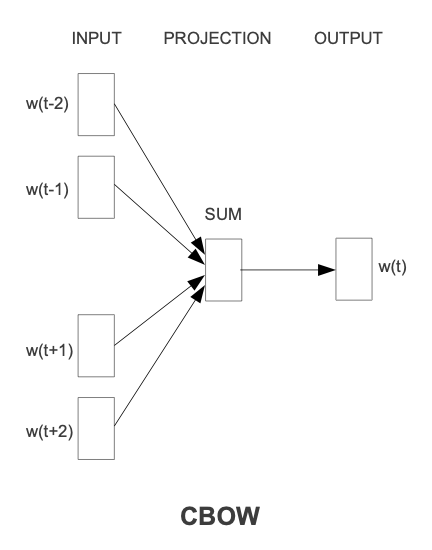
\includegraphics[width=0.4\textwidth]{../img/cbow.png}
	\caption{CBOW model \citep{mikolov2013efficient}.}
	\label{cbow}
\end{figure}
 \newpage
\subsection{(Distil)BERT for single sequence classification}

Transformer networks took the world by storm due to its paralellization capabilities and toppled established architectures such as LSTMs with new state of the art scores in several NLP tasks. While a traditional transformer has encoder and decoder blocks, Bidirectional Encoder Representation from Transformers (BERT), as the name suggests, only has encoder blocks \citep{halthor2020}. The BERT architecture is pre-trained with huge corpora such the BookCorpus (800M words) and English Wikipedia (2,500M words) \citep{devlin2019bert}.

BERT uses two techniques simultaneously for pre-training: Masked Language Model (MLM) and Next Sentence Prediction (NSP). The former consists into masking out a certain amount of words from sentences and training to predict those words, e.g. "The corona [MASK] outbreak" and the prediction of the word "virus". The latter is the task of judging if a sentence is a continuation of a previous sentence, e.g. The sentence "Voted in Nicaraguan elections" does \textit{not} follow the sentence "The penguins of Antartica." The first task is responsible to train context \textit{within} the sentence, while the second task trains context between sentences.

Every sequence in BERT has the special [CLS] token as the first token (see Figure~\ref{fig-cls}). Additionally, every BERT input embedding, $\mathit{E}$, is the sum of three different embeddings: token, segment, and position. The token embedding is retrieved from the pre-trained WordPiece embeddings, with a 30,000 token vocabulary. The segment embeddings encode which sequence it is dealing with (sequence A or B in a NSP task). Finally, the positional embedding is encodes a word's position in that sentence. This embedding \textit{E} is then fed into the network and the last hidden state of the [CLS] token can be seen as agregate sequence representation that can be used for classification \citep{devlin2019bert} as seen on Figure~\ref{fig-bert}.

\begin{figure}[!h]
	\centering
	\subfloat[]{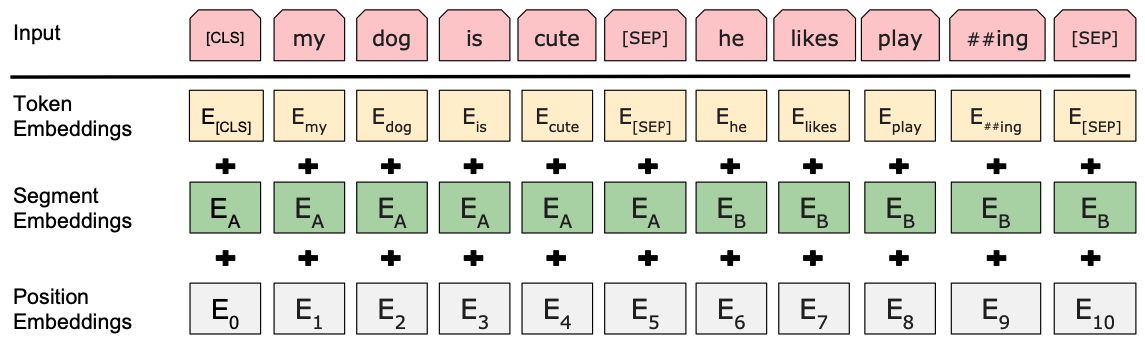
\includegraphics[width=0.6\textwidth]{../img/embeddings.png}\label{fig-cls}}
	\hfill
	\subfloat[]{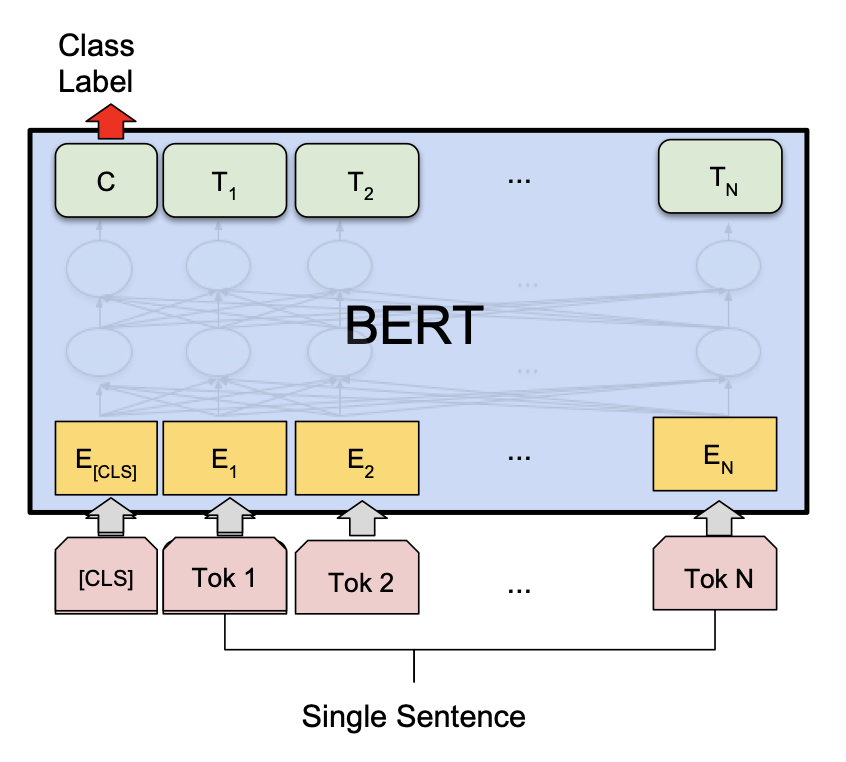
\includegraphics[width=0.4\textwidth]{../img/BERT-class.png}\label{fig-bert}}
	\caption{(a) BERT's input representation and (b) BERT for single sequence classification \citep{devlin2019bert}.}
\end{figure}



The distilBERT model is a case of transfer learning technique called distillation where a "student" model is trained to achieve  the behaviour of a larger "teacher" model \citep{sanh2020distilbert}. This managed to "reduce the size of a BERT model by 40\%, while retaining 97\% of its language understanding capabilities and being 60\% faster" \citep{sanh2020distilbert}.



\subsection{Linear Support Vector Classification}

Given pairs of observations -- word embeddings -- and labels -- sarcastic or not -- $(\mathbf{x}_i, y_i)$, a support vector classifier tries to find the hyperplane which maximizes the margins between classes \citep{pena2019}. The kernel used in classification can vary, but for NLP applications where the numbers of features are large, the linear kernel is more suitable given that text data is often linearly separable and the computations are faster \citep{hsu2003}. The prediction is given by Equation~\ref{eqn:svm} and  the maximum margin is given by Equation~\ref{eqn:margin} \citep{pena2019} 

\begin{equation}
	\label{eqn:svm}
 	\hat{y}= \mathbf{xw} +  b
\end{equation}

\begin{equation}
	\label{eqn:margin}
	argmax_{\mathbf{w}, b} \frac{1}{||\mathbf{w}||}
\end{equation}

